\documentclass[a4paper,10pt]{article}
\usepackage[utf8]{inputenc}
\usepackage[nottoc,numbib]{tocbibind} % makes the BibTeX references section appear in the table of contents
\usepackage[inline]{enumitem}
\usepackage{amssymb}
\usepackage{amsfonts}
\usepackage{amsmath}
\usepackage{amsthm}
\usepackage{color}
\usepackage{caption}
\usepackage{subcaption}
\usepackage{graphicx}
\usepackage{mathtools}
\usepackage{mathrsfs}
\usepackage{framed}
% eventually make left/right margins equal
\usepackage[top=0.6in,bottom=0.6in,left=0.1in,right=0.9in]{geometry}
\usepackage{dsfont}



\usepackage[textwidth=0.7in]{todonotes}

\usepackage[hidelinks]{hyperref} %this needs to be loaded last!

% for 3D pictures
\usepackage{tikz}
\usepackage{tikz-3dplot}
\usetikzlibrary{perspective}
\tdplotsetmaincoords{82}{20}

% for arrow/commutative diagrams
\usepackage{tikz-cd}

%prevent math mode statements from being broken up across lines
\relpenalty=9999
\binoppenalty=9999

%claim environment
\newenvironment{claim}[1]{\par\noindent\underline{Claim:}\space#1}{}

%leftbar
\renewenvironment{leftbar}[1][\hsize]
{%
    \def\FrameCommand
    {%
        {\vrule width 3pt}%
        \hspace{0pt}%must no space.
        \fboxsep=\FrameSep\colorbox{white}%
    }%
    \MakeFramed{\hsize#1\advance\hsize-\width\FrameRestore}%
}
{\endMakeFramed}

% fix footnote spacing
\let\oldfootnote\footnote
\renewcommand{\footnote}{\unskip\oldfootnote}


%numbering and style of theorems
\theoremstyle{plain}
\newtheorem{Theorem}{Theorem}
\newtheorem{Proposition}[Theorem]{Proposition}
\newtheorem{Corollary}[Theorem]{Corollary}
\newtheorem{Lemma}[Theorem]{Lemma}
\newtheorem{Question}[Theorem]{Question}
\newtheorem{Conjecture}[Theorem]{Conjecture}
\newtheorem{Assumption}[Theorem]{Assumption}
\newtheorem{Algorithm}[Theorem]{Algorithm}

\theoremstyle{definition}
\newtheorem{Definition}[Theorem]{Definition}
\newtheorem{Property}[Theorem]{Property}
\newtheorem{Notation}[Theorem]{Notation}
\newtheorem{Condition}[Theorem]{Condition}
\newtheorem{Example}[Theorem]{Example}
\newtheorem{Exercise}[Theorem]{Exercise}
\newtheorem{Introduction}[Theorem]{Introduction}

\theoremstyle{remark}
\newtheorem{Remark}[Theorem]{Remark}
\newtheorem{case}{Case}[Theorem]

% make proofs use filled in black square instead of empty square
\renewcommand{\qedsymbol}{$\blacksquare$}
%\renewcommand\proof{\noindent\textit{\textbf{Proof. }}}
\newcommand{\modo}[3]{#1 \equiv #2 \pmod{#3}}
\newcommand{\nmodo}[3]{#1 \not\equiv #2 \pmod{#3}}
\newcommand{\R}{\mathbb{R}}
\newcommand{\Q}{\mathbb{Q}}
\newcommand{\N}{\mathbb{N}}
\newcommand{\Z}{\mathbb{Z}}
\newcommand{\Zpos}{\mathbb{Z}_{\geq 0}}
\renewcommand{\vec}[1]{\mathbf{#1}}
\newcommand{\dist}{\text{dist}}
\newcommand{\F}{\mathbb{F}}
\newcommand{\C}{\mathbb{C}}
\newcommand{\lin}{\text{lin}}
\newcommand{\cl}{\text{cl}}
\newcommand\norm[1]{\left\lVert#1\right\rVert}
\newcommand{\ONE}{\mathds{1}}
\newcommand{\generatedby}[1]{\left\langle#1\right\rangle}
\newcommand{\id}{\text{id}}
\DeclareMathOperator{\sgn}{sgn}
\newcommand\abs[1]{\left|#1\right|}
\newcommand\Gl{\text{Gl}}
\DeclareMathOperator{\pam}{pam}
%lifted point array
\newcommand{\lpa}[1]{\Sigma({#1})}

\title{Virus Research \\ \large SIP}
\author{Xavier Silva}

\begin{document}

\maketitle

\tableofcontents

% \newpage

\section{Abstract}

Icosahedral viruses have the symmetries of an icosahedron, which involves 2-fold, 3-fold, and 5-fold rotational symmetries.
We can approximate these virus capsids with finite sets of points (called a point array) which we realize in 6D (not just 3D) for the purpose of crystallography: our 6D point arrays naturally fit inside 6D icosahedral lattices. There are \(55\) standard point arrays (called \emph{one-base}) from which we build all the others.
We model virus maturation by 6D linear transformations (transitions) of point arrays that preserve some or all of icosahedral symmetry.
The symmetries we wish to preserve are either full icosahedral, $A_4$ ($3$-fold and $2$-fold), $D_{10}$ ($5$-fold and $2$-fold) or $D_6$ ($3$-fold and $2$-fold) symmetry.
We define full icosahedral symmetry as a group defined by \(\mathcal{I} := \generatedby{a, b | a^2 = b^3 = (ab)^5 = 1}\).
We then notice that \(A_4, D_{10}, \text{ and } D_6\) are maximal subgroups of \(\mathcal{I}\).
To find transitions that preserve one of these symmetry groups, we solve matrix equations of the form \(TB_0 = B_1\) for \(T\), where \(T\) is a \(6\times6\) matrix that depends on either 2, 4, 6, or 8 real variables, depending on which symmetry we are looking at and \(B_0\) and \(B_1\) are representations of the point arrays.
Note that actually finding transitions requires a large amount of computation.
From this we are able to reproduce previously discovered transitions for the Cowpea Chlorotic Mottle Virus that preserve \(D_6\) symmetry, and more importantly create a comprehesive list of what symmetries can be preserved between any possible combination of the \(55\) standard point arrays.

\section{Intro}
Icosahedral viruses have the symmetries of an icosahedron, which involves 2-fold, 3-fold, and 5-fold rotational symmetries.
We can approximate these virus capsids with finite sets of points (called a point array) which we realize in 6D (not just 3D) for the purpose of crystallography: our 6D point arrays naturally fit inside 6D icosahedral lattices. 
There are \(55\) standard point arrays (called \emph{one-base}) from which we build all the others.
We model virus maturation by 6D linear transformations (transitions) of point arrays that preserve some or all of icosahedral symmetry.


% Viruses have a point cloud, we can then lift into 6D dimensions in a non-trivial way.
% These point clouds will then fit into a \emph{lattice}.

Relevant to our work the shape of the icosahedron, a shape with 2-fold, 3-fold, and 5-fold symmetry.
\begin{Definition}[Icosahedral Group]
	The icosahedral group, which we denote by \(\mathcal{I}\), is the 60-element group given by \[\mathcal{I} := \generatedby{a, b | a^2 = b^3 = (ab)^5 = 1}.\]
\end{Definition}
\noindent We realize the icosahedral group as a \( 6 \times 6 \) matrix group.
\begin{Definition}[Generators of the Icosahedral Group]
	A 6D representation of the generators for \(\mathcal{I}\) are as follows:
	\[a = \begin{bmatrix}
		-1 & 0  & 0 & 0 & 0 & 0 \\
		0  & -1 & 0 & 0 & 0 & 0 \\
		0  & 0  & 0 & 0 & 1 & 0 \\
		0  & 0  & 0 & 0 & 0 & 1 \\
		0  & 0  & 1 & 0 & 0 & 0 \\
		0  & 0  & 0 & 1 & 0 & 0
	\end{bmatrix} \quad b = \begin{bmatrix}
		0 & -1 & 0  & 0 & 0 & 0 \\
		0 & 0  & -1 & 0 & 0 & 0 \\
		1 & 0  & 0  & 0 & 0 & 0 \\
		0 & 0  & 0  & 0 & 0 & 1 \\
		0 & 0  & 0  & 1 & 0 & 0 \\
		0 & 0  & 0  & 0 & 1 & 0
	\end{bmatrix}.\]
\end{Definition}

The icosahedral group has 3 maxmial subgroups, which we call \( A_4 \), \( D_{10} \), and \( D_6 \).
These maximal subgroups represent the symmetries of the tetrahedron, pentagonal prism, and triangular prism respectively.
This is shown in figure \ref{fig:maximal_subgroups}.
Notice that these shapes can fit within the icosahedron.
These maximal subgroups are subsets of \( \mathcal{I} \) that are themselves groups.
\footnote{Like the icosahedral group, these subgroups are generated by two \( 6 \times 6 \) matrices.}
In a way, the maximal subgroups represent subsets of symmetries of the icosahedron.
% maximal subgroup figures
\begin{figure}[h]
	\captionsetup{width=0.75\textwidth}
	\centering
	% A4
	\begin{tikzpicture}[scale=0.5, tdplot_main_coords,
		declare function={b=5;h=4.33;l=15;}]
		\draw[fill=gray,fill opacity=0.3] (b/2,-l/2,0)  -- (0,-l/2,h) -- (-b/2,-l/2,0) -- cycle;
		% \draw (b/2,-l/2,0) -- (0, l-20, h/3);
		% \draw (0,-l/2,h) -- (0, l-20, h/3);
		% \draw (-b/2,-l/2,0) -- (0, l-20, h/3);
		\draw (b/2,-l/2,0) -- (0, 0, h/3);
		\draw (0,-l/2,h) -- (0, 0, h/3);
		\draw[dashed] (-b/2,-l/2,0) -- (0, 0, h/3);
		\draw[orange,dashed] (0,-l/2,h/3) -- (0,l/2,h/3); % center to center aka 3 fold
		\draw[orange] (0,-l/2-10,h/3) -- (0,-l/2,h/3);
		% \node[fill=orange, circle, inner sep=4pt] at (0,-l/2,h/3) {};
		\draw[blue, dashed] (0, -l/4, 4*h/6) -- (0,-l/2,0);
		\draw[blue] (0, -l/4, 4*h/6) -- (0, -l/4+1/8*l, {4*h/6+1/8*(2*h+3)});
		\draw[blue] (0,-l/2,0) -- (0,-l/2-1/10*l,{-1/10*(2*h+3)});
		
		%draw the axes
		% \draw[red] (0,0,0) -- (3,0,0) node[anchor=west]{$x$};
		% \draw[green] (0,0,0) -- (0,3,0) node[anchor=west]{$y$};
		% \draw[blue] (0,0,0) -- (0,0,3) node[anchor=west]{$z$};
	\end{tikzpicture}
	% D10
	\begin{tikzpicture}[scale=0.4, tdplot_main_coords,
		declare function={r=3;l=5;}]
		% \draw ({r*cos(0)}, l, {r*sin(0)}) -- ({r*cos(72)}, l, {r*sin(72)}) -- ({r*cos(144)}, l, {r*sin(144)}) -- ({r*cos(216)}, l, {r*sin(216)}) -- ({r*cos(288)}, l, {r*sin(288)});
		
		% front face
		\draw[fill=gray,fill opacity=0.3] ({r*cos(18)}, -l, {r*sin(18)}) -- ({r*cos(90)}, -l, {r*sin(90)}) -- ({r*cos(162)}, -l, {r*sin(162)}) -- ({r*cos(234)}, -l, {r*sin(234)}) -- ({r*cos(306)}, -l, {r*sin(306)}) -- cycle;
		
		% back face
		\draw ({r*cos(18)}, l, {r*sin(18)}) -- ({r*cos(18+72)}, l, {r*sin(18+72)});
		\draw[dashed] ({r*cos(90)}, l, {r*sin(90)}) -- ({r*cos(90+72)}, l, {r*sin(90+72)});
		\draw[dashed] ({r*cos(162)}, l, {r*sin(162)}) -- ({r*cos(162+72)}, l, {r*sin(162+72)});
		\draw ({r*cos(234)}, l, {r*sin(234)}) -- ({r*cos(234+72)}, l, {r*sin(234+72)});
		\draw ({r*cos(306)}, l, {r*sin(306)}) -- ({r*cos(306+72)}, l, {r*sin(306+72)});
		
		% connect front and back faces
		\draw ({r*cos(18)}, l, {r*sin(18)}) -- ({r*cos(18)}, -l, {r*sin(18)});
		\draw ({r*cos(90)}, l, {r*sin(90)}) -- ({r*cos(90)}, -l, {r*sin(90)});
		\draw[dashed] ({r*cos(162)}, l, {r*sin(162)}) -- ({r*cos(162)}, -l, {r*sin(162)});
		\draw[dashed] ({r*cos(234)}, l, {r*sin(234)}) -- ({r*cos(234)}, -l, {r*sin(234)});
		\draw ({r*cos(306)}, l, {r*sin(306)}) -- ({r*cos(306)}, -l, {r*sin(306)});
		
		% 2-fold axis
		\draw[blue] (0,0,r+2) -- (0,0,r);
		\draw[blue, dashed] (0,0,r) -- (0,0,-r);
		\draw[blue] (0,0,-r) -- (0,0,-r-1);
		
		% 5-fold axis
		\draw[orange, dashed] (0, l+2*r, 0) -- (0, -l, 0);
		\draw[orange] (0, -l, 0) -- (0, -l-3*r, 0);
		
		%draw the axes
		% \draw[red] (0,0,0) -- (3,0,0) node[anchor=west]{$x$};
		% \draw[green] (0,0,0) -- (0,3,0) node[anchor=west]{$y$};
		% \draw[blue] (0,0,0) -- (0,0,3) node[anchor=west]{$z$};
	\end{tikzpicture}
	% D6
	\begin{tikzpicture}[scale=0.4, tdplot_main_coords,
		declare function={b=5;h=4.33;l=15;}]
		\draw[dashed] (-b/2,-l/2,0) -- (-b/2,l/2,0) edge (b/2,l/2,0) -- (0,l/2,h);     
		\draw (b/2,l/2,0) -- (0,l/2,h) -- (0,-l/2,h);
		\draw[fill=gray,fill opacity=0.3] (b/2,-l/2,0)  -- (0,-l/2,h) -- (-b/2,-l/2,0);
		\draw (b/2,-l/2,0)  -- (b/2,l/2,0);
		\draw (b/2,-l/2,0)  --   (-b/2,-l/2,0);
		% \draw (0,-l/2,0)  --  (0,-l/2,h);
		\draw[orange,dashed] (0,-l/2,h/3) -- (0,l/2+5,h/3); % center to center aka 3 fold
		\draw[orange] (0,-l/2-10,h/3) -- (0,-l/2,h/3);
		% \node[fill=orange, circle, inner sep=3pt] at (0,-l/2,h/3) {};
		% \node[draw=orange, circle, inner sep=3pt] at (0,l/2,h/3) {};
		
		\draw[blue] (0,0,h+2) -- (0,0,h); % top to bottom aka 2 fold
		\draw[blue, dashed] (0,0,h) -- (0,0,-1.1); % top to bottom aka 2 fold
		\draw[blue] (0,0,-1.1) -- (0,0,-2);
		
		%draw the axes
		% \draw[red] (0,0,0) -- (3,0,0) node[anchor=west]{$x$};
		% \draw[green] (0,0,0) -- (0,3,0) node[anchor=west]{$y$};
		% \draw[blue] (0,0,0) -- (0,0,3) node[anchor=west]{$z$};
	\end{tikzpicture}
	\caption{
		A visual representation of the maximal subgroups. From left to right we have \(A_4\), \(D_{10}\), and \(D_6\). 
		The 2-fold axes are labeled in blue while the 3-fold and 5-fold axes are labeled in orange.
		Note that \( A_4 \) has multiple 2-fold and 3-fold axes (by rotating the labeled axes) while \( D_6 \) only has one 2-fold and 3-fold axis.
	}
	\label{fig:maximal_subgroups}
\end{figure}
\section{Point Arrays and Lattices}
Icosahedral viruses are characterized by point arrays, which are a set of points in 3 dimensions.
\begin{Definition}[Lifted Point Array]
	Let \(\vec{t}, \vec{v}_1, \vec{v}_2, \dots, \vec{v}_n\) be 6 dimensional vectors.
	Then the lifted point array generated by these vectors is \[\lpa{\vec{t}, \vec{v}_1, \vec{v}_2, \dots, \vec{v}_n} := \mathcal{I}\vec{v}_1 \cup \mathcal{I}\vec{v}_2 \cup \dots \cup \mathcal{I}\vec{v}_n \cup (\mathcal{I}\vec{v}_1 + \mathcal{I}\vec{t}) \cup (\mathcal{I}\vec{v}_2 + \mathcal{I}\vec{t}) \cup \dots \cup (\mathcal{I}\vec{v}_n + \mathcal{I}\vec{t}).\]
\end{Definition}
Notice that while icosahedral viruses are characterized by 3 dimensional point arrays, \emph{lifted point arrays} are 6 dimensional.
This is because we want lifted point arrays to fit inside icosahedral lattices, and no such lattices exist in dimensions lower than 6.
\footnote{Because lattices of dimension 5 and lower cannot preserve 5-fold rotational symmetry.}
However, we can project lifted point arrays from 6 dimensions into 3 dimensions using the projection matrix given in \cite{indelicatoetal2012}.

There are 55 standard point arrays from which we build all others.
These are called the \emph{one-base} point arrays and take the form \(\mathcal{I}\vec{v} \cup (\mathcal{I}\vec{v} + \mathcal{I}\vec{t})\). This form tells us that only one translation vector and one ``base" vector is needed to create the point array. \cite{keeftwarock2009affine}

Here we define these one-base point arrays with two vectors, a translation and base vector.
However, we could define the same point array with more than two vectors, if we added on a vector from the base vector's icosahedral orbit.
Thus if \( \vec{u} \in \mathcal{I}\vec{v} \) we would have that 
\todo{perhaps add more of a proof to this? Group actions and orbits would be needed here}
\begin{equation}
	\mathcal{I}\vec{v} \cup (\mathcal{I}\vec{v} + \mathcal{I}\vec{t}) = \mathcal{I}\vec{v} \cup \mathcal{I}\vec{u} \cup (\mathcal{I}\vec{v} + \mathcal{I}\vec{t}) \cup (\mathcal{I}\vec{u} + \mathcal{I}\vec{t})
	\label{eq:example-for-generating-tuples}
\end{equation}
Therefore we have many ways of talking about the same point array. 
\begin{Definition}[Minimal Generating Tuple]
	A tuple of six dimensional vectors $ (\vec{t}, \vec{v}_1, \vec{v}_2, ... , \vec{v}_{n})$ is a \emph{minimal generating tuple}  and the union 
	\[
	\lpa{\vec{t}, \vec{v}_1, \vec{v}_2, ... , \vec{v}_{n}}: = \left(\bigcup_{i=1}^{n} \mathcal{I} \; \vec{v}_i \right) \cup \left( \bigcup_{i=1}^{n} \mathcal{I} \; \vec{v}_i + \mathcal{I} \; \vec{t} \right) 
	\]
	is called the \textbf{($\mathbf{n}$-base) lifted point array} generated by this tuple so long as 
	\begin{enumerate}
		\item Each of the vectors $\vec{t}$, $\vec{v}_i$ in the tuple points along a $2$-fold, $3$-fold or $5$-fold rotational axis of the action of $\mathcal{I}$.
		\item The orbits $\mathcal{I} \; \vec{v}_i$, $\; 1 \leq i \leq n$, are all distinct.
		\item $\displaystyle 
		|\lpa{\vec{t}, \vec{v}_1, \vec{v}_2, ... , \vec{v}_{n}}| < \sum_{i=1}^{n} | \mathcal{I} \; \vec{v}_i| + | \mathcal{I} \; \vec{v}_i|| \mathcal{I} \; \vec{t}|. 
		$ \todo{Ask Dr. Oloo about this condition}
	\end{enumerate}
\end{Definition}
\begin{Definition}[Generating Tuple]
	More generally, a tuple $ (\vec{t}, \vec{v}_1, \vec{v}_2, ... , \vec{v}_{n})$ is a \emph{generating tuple} if it has a sub-tuple $ (\vec{t}, \vec{v}_{i_1}, \vec{v}_{i_2}, ... , \vec{v}_{i_m})$, $1 \leq i_1 < i_2 < ... < i_m \leq n$, that is a minimal generating tuple and the unions
	\[
	\lpa{\vec{t}, \vec{v}_1, \vec{v}_2, ... , \vec{v}_{n}}: = \left(\bigcup_{i=1}^{n} \mathcal{I} \; \vec{v}_i \right) \cup \left( \bigcup_{i=1}^{n} \mathcal{I} \; \vec{v}_i + \mathcal{I} \; \vec{t} \right) 
	\]
	and $\lpa{\vec{t}, \vec{v}_{i_1}, \vec{v}_{i_2}, ... , \vec{v}_{i_m}}$ are equal.
\end{Definition}
% above two definitions are from Dr. Oloo
These definitions allow us to distinguish between the two cases given in equation \ref{eq:example-for-generating-tuples}.
The tuple \( (\vec{t}, \vec{v}) \) is the minimal generating tuple and the tuple \( (\vec{t}, \vec{v}, \vec{u}) \) is simply a generating tuple (assuming \( \vec{u} \in \mathcal{I}\vec{v} \)).

\subsection{Constructing Point Arrays}
Constructing a one-base point array involves us finding all vectors in the set \(\mathcal{I}\vec{v} \cup (\mathcal{I}\vec{v} + \mathcal{I}\vec{t})\).
This is shown visually in figure \ref{fig:point_array_construction}.

\begin{figure}[h!]
	\centering
	\begin{subfigure}{0.25\textwidth}
		\centering
		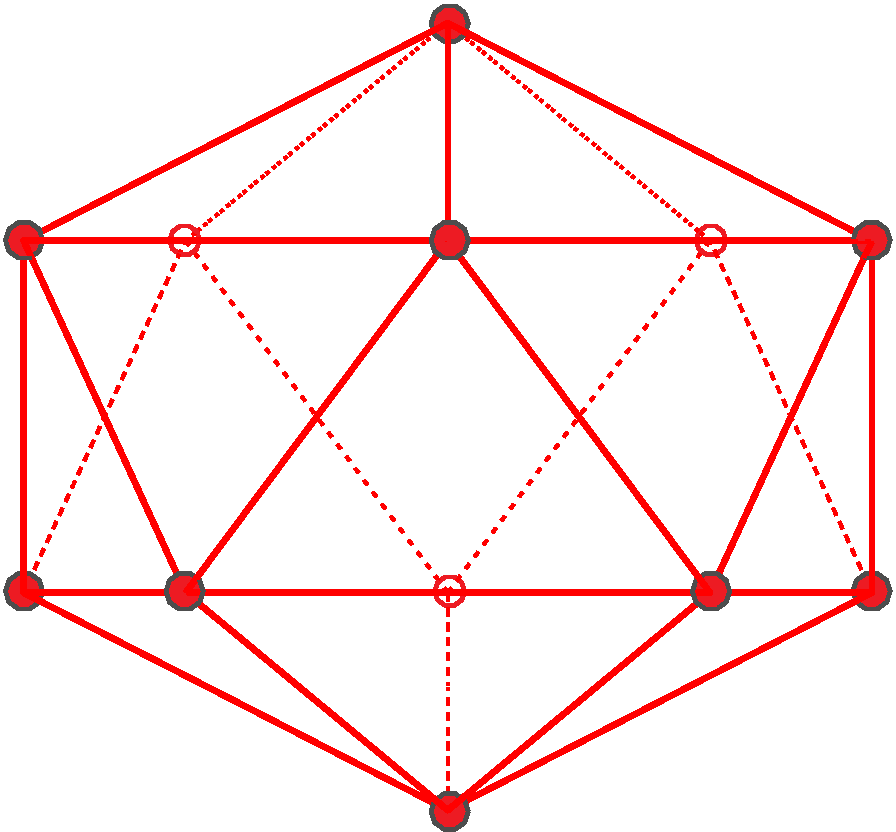
\includegraphics[width=\textwidth]{images/p_arr_construction_1.pdf}
		\caption{Start with icosahedron, created by applying icosahedral symmtry on one vector. Mathematically this is \(\mathcal{I}\vec{v}\).}
	\end{subfigure}
	\hfill
	\begin{subfigure}{0.3\textwidth}
		\centering
		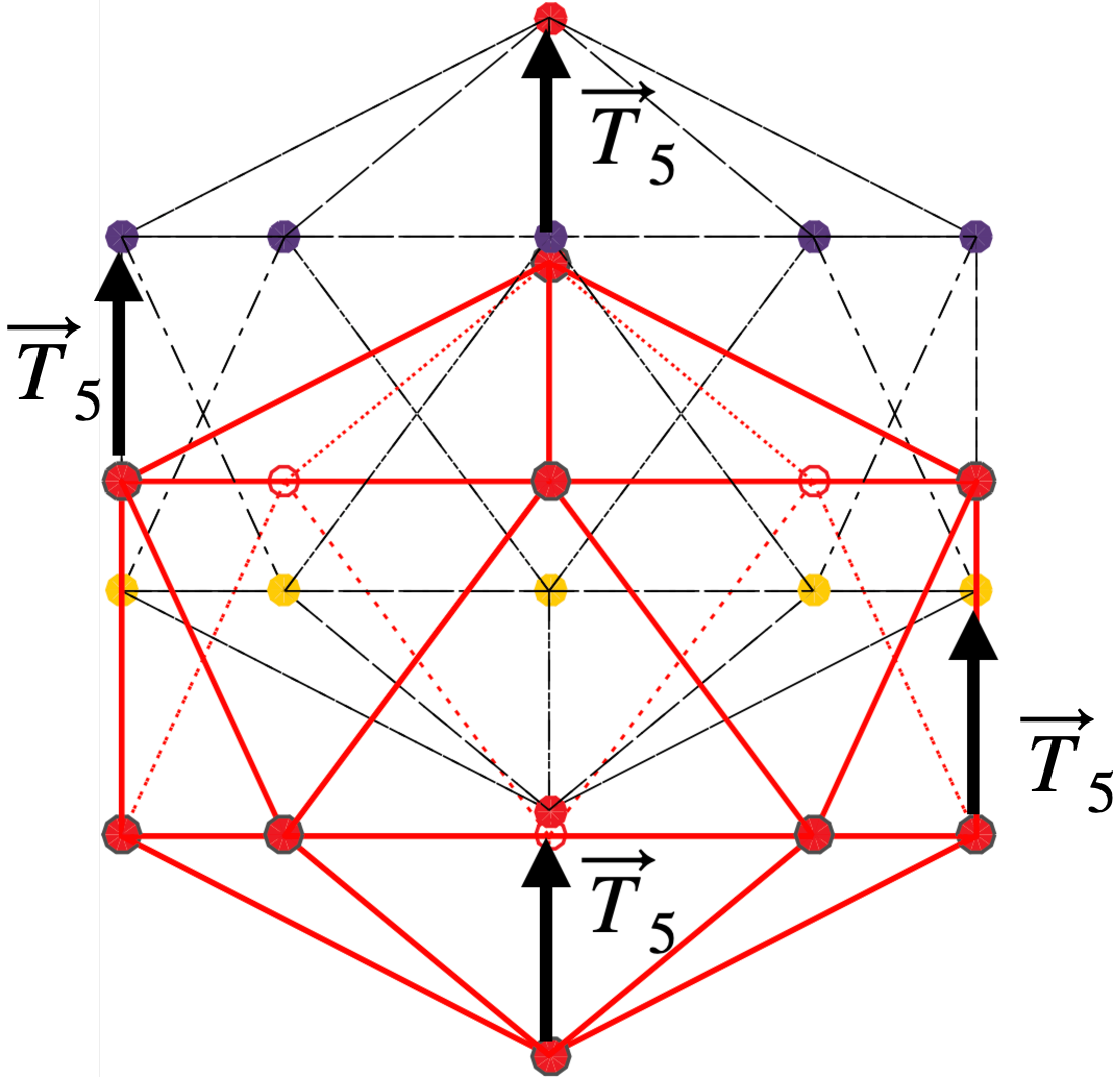
\includegraphics[width=\textwidth]{images/p_arr_construction_2.pdf}
		\caption{Shift icosahedron by a translation vector. In this example we are translating along the 5-fold axis of the icosahedron. Mathematically this is \mbox{\(\mathcal{I}\vec{v} \cup (\mathcal{I}\vec{v} + \vec{t})\)}.}
	\end{subfigure}
	\hfill
	\begin{subfigure}{0.35\textwidth}
		\centering
		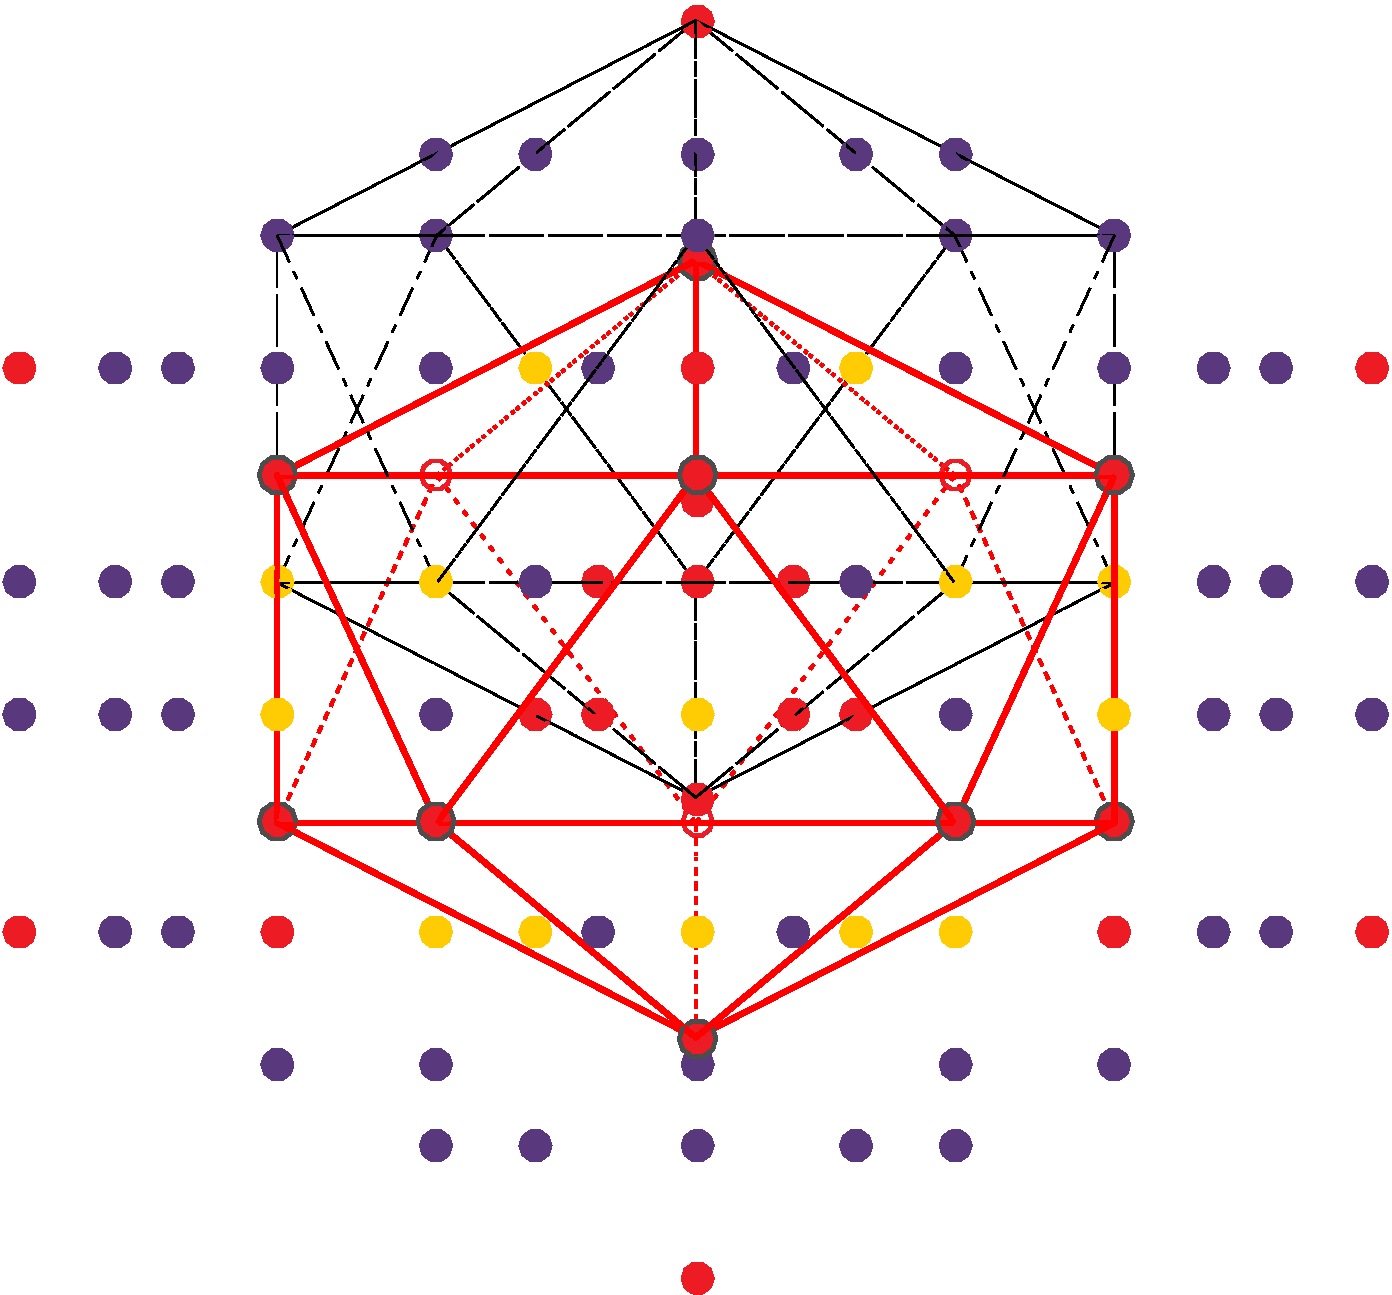
\includegraphics[width=\textwidth]{images/p_arr_construction_3.pdf}
		\caption{Reapply icosahedral symmetry, getting the final expression \(\mathcal{I}\vec{v} \cup (\mathcal{I}\vec{v} + \mathcal{I}\vec{t})\).}
	\end{subfigure}
	\caption{The process of creating a one-base point array. Graphics from Dr. Dave Wilson.}
	\label{fig:point_array_construction}
\end{figure}

\section{Transitions Between Point Arrays}
Let us take an overall look at how we wish to use point arrays.
Viruses are characterized by 3-dimensional point arrays.
We want our point arrays to represent the symmetry and structure of the virus.
Then we lift the point arrays into 6 dimensions, because we the point array to fit inside an icosahedral lattice.
Lattices on a general level encode symmetry.
When our point arrays fit inside lattices, we can use knowledge about lattices in order to describe symmetry of the point array.
\todo{Add citation}
Point arrays let us look at the most important structural points of a virus and can determine what potential modifications could be done to a particular virus.

With point arrays, we can try to find linear transformations to map one point array onto another.
In general, finding such a linear map is relatively easy.
A more difficult challenge is to find such a linear map that preserves symmetry.
Our point arrays have icosahedral symmetry.
Therefore our desire is to find a linear map from one point array to another where the intermediate point arrays also have icosahedral symmetry.
It may also be desirable to find a map that preserves a looser symmetry that fits inside icosahedral symmetry.

Additionally, instead of mapping the point arrays directly onto each other, our linear transformations will transform one lattice into another.
The consequence of doing this is that when we restrict our map to the point array, it becomes a map from one point array to another.

The process of mathematically describing these symmetry preserving maps and how we find them will be the focus of the rest of this paper.
\subsection{Viral Maturation}
Icosahedral viruses mature over time, and maturation is how they become infectous.
For this paper we will focus on the Cowpea Chlorotic Mottle Virus (CCMV).
This virus is characterized by one of the standard point arrays.
How CCMV matures is shown by figure \ref{fig:CCMV_maturation}.
Notice the points in orange, these points collectively are the point arrays that characterize the CCMV virus.
We wish to see if there exists a linear transformation that maps the native point array to the mature point array while preserving icosahedral symmetry (or one of its maximal subgroups).

\begin{figure}[!h]
	\centering
	\captionsetup{width=0.5\textwidth}
	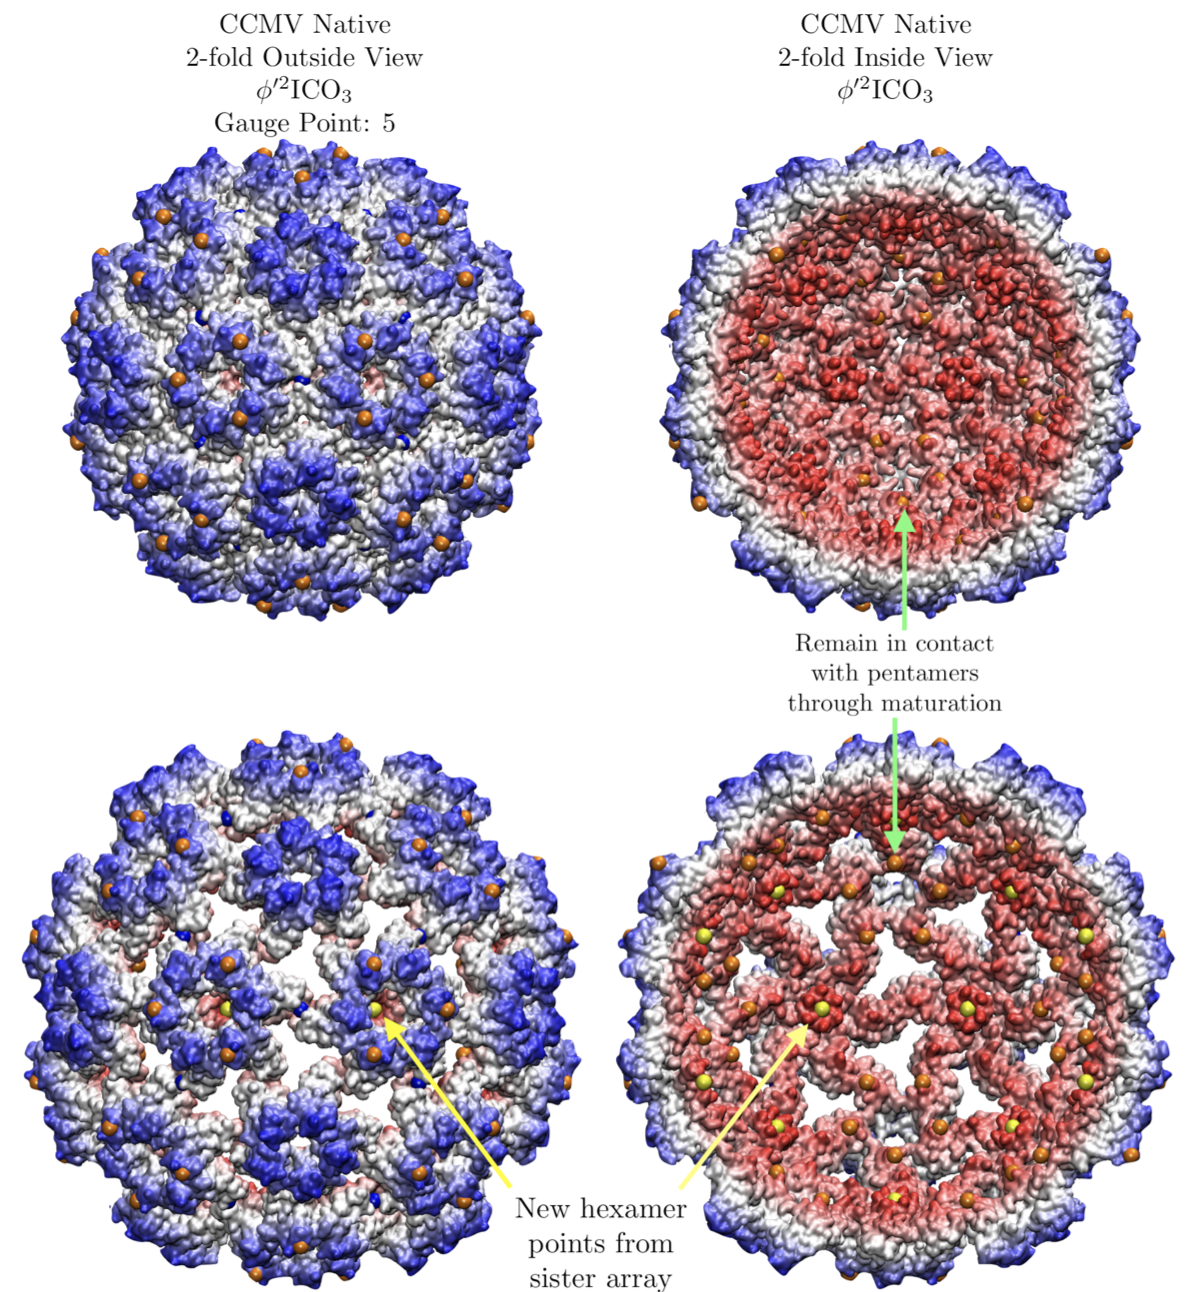
\includegraphics[width=0.5\textwidth]{images/CCMV_maturation.png}
	\caption{
		The above diagram shows CCMV in its native state (first row) and mature state (second row). 
		Notice the points in orange are the points that characterize CCMV.
		Graphics from Dr. Dave Wilson.
	}
	\label{fig:CCMV_maturation}
\end{figure}

\section{Mathematical View of the Problem}
Our desire to find transitions between point arrays that preserving some or all of icosahedral symmetry.
In order to find such transitions, we need to understand this problem mathematically.
On the highest level of abstraction, we are simply solving matrix equations of the form \[TB_0 = B_1.\]
In this equation, \(B_0\) and \(B_1\) represent the native and mature point arrays respectively, and \(T\) is our desired linear transformation that preserves icosahedral symmetry.
\footnote{Recall that we realize icosahedral symmetry as a matrix group and lifted point arrays are sets of vectors, so it makes sense that we are solving a matrix equation.}
Because we want to represent the point arrays, there is a specific structure to the \( B_0 \) and \( B_1 \) matrices.
Let us call us these matrices \emph{point array matrices}.
Before we define a point array matrix, we introduce a new notation called \emph{bar notation}.
\newcommand{\icobar}[1]{\overline{\vec{#1}}}

\begin{Definition}[Icosahedral Bar Notation]
	%\newcommand{\icobar}[2]{\overline{\vec{#1}_{#2}}}
	Let \(\vec{v}\) be a 6-dimensional vector.
	Then we define that \(\icobar{v}\) is an element of the icosahedral orbit of \(\vec{v}\).
	That is, \(\icobar{v} \in \mathcal{I}\vec{v}\).
	\todo[inline, color=yellow]{Not entirely sure about this icobar notation}
\end{Definition}
This definition allows us to easily denote when we wish to represent an element of the icosahedral orbit of a vector.
With this notation in hand, we can now define a point array matrix.
\begin{Definition}[Point Array Matrix]
	Let \(P\) be a given point array.
	\( P \) is generated by vectors \(\vec{t}, \vec{v}_1, \vec{v}_2, \dots, \vec{v}_n\).
	\todo[color=red]{fix the bold face in subscript of \texttt{icobar} command}
	A \emph{point array matrix} is a \( 6 \times (n+1) \) matrix of the form \[\begin{bmatrix}
		| & | & | & \cdots & | \\
		\icobar{t} & \icobar{v_1} & \icobar{v_2} & \cdots & \icobar{v_n} \\
		| & | & | & \cdots & | 
	\end{bmatrix}\]
	whose rank is either equal to the minimum of \( n+1 \) and 6.
	Notice that because we are using the icosahedral bar notation defined earlier, this definition is representing a class of matrices that all correspond to the same point array.
	That is, we are defining the form of any representative of the given point array \( P \).
	Denote the set of point array matrices for \( P \) as \( \pam(P) \).
\end{Definition}
The \( B_0 \) and \( B_1 \) matrices are both point array matrices and so both have this general form for their respective point arrays.

One fact that will be useful to know is how many point array matrices there are for a singular point array.
Let \( P \) be a point array.
If we let \( m \) be the number of point array matrices for \( P \) then
\[m \leq \abs{\mathcal{I}\vec{t}} \cdot \abs{\mathcal{I}\vec{v}_1} \cdot \abs{\mathcal{I}\vec{v}_2} \cdot \dots \cdot \abs{\mathcal{I}\vec{v}_n}.\]
We can only say for certain that \( m \) is less than or equal to this value because we require point array matrices to be linearly independent (or have rank 6).
\footnote{If we have that \( \vec{v}_i = \vec{v}_j \) with \( i \neq j \), then there are matrices of the correct form that are not linearly independent.}
However, in general we can assume that \( m \) is equal to this value since in general all the generating vectors are distinct.

\subsection{Mathematically Describing Transitions}
We have defined what the \( B_0 \) and \( B_1 \) matrices look like, now we define the nature of the \( T \) matrix.
A transition \(T\) that preserves all of icosahedral symmetry must have the form: \begin{equation} \label{eq:ico-transition}
	T = \begin{bmatrix}
		z  & x  & -x & -x & x  & x \\
		x  & z  & x  & -x & -x & x \\
		-x & x  & z  & x  & -x & x \\
		-x & -x & x  & z  & x  & x \\
		x  & -x & -x & x  & z  & x \\
		x  & x  & x  & x  & x  & z
\end{bmatrix}\end{equation}

Our linear transformation \(T\) preserves icosahedral symmetry because it is in the centralizer of \(\mathcal{I}\) (or one its of maximal subgroups).
\begin{Definition}[Centralizer]
	The centralizer of a group \(G\), denoted by \(Z(G)\) is the set of elements that commute with all elements of \(G\).
	That is, \[Z(G) = \{z\ |\ gz = zg\ \forall g \in G\}.\]
\end{Definition}
Any matrix of the form given in equation \ref{eq:ico-transition} is in \(Z(\mathcal{I})\), the centralizer of \(\mathcal{I}\).
Below are the general matrix forms for \(Z(A_4)\), \(Z(D_{10})\), and \(Z(D_6)\). \cite{indelicatoetal2012}
\begin{align}
	\begin{bmatrix}
		z  & -x & -y & -t & t  & -x \\
		t  & z  & t  & x  & x  & y  \\
		-y & -x & z  & t  & -t & -x \\
		x  & -t & -x & z  & y  & t  \\
		-x & -t & x  & y  & z  & t  \\
		t  & y  & t  & -x & -x & z
	\end{bmatrix} \in Z(A_4) \\
	\begin{bmatrix}
		z & x & y & y & x & t \\
		x & z & x & y & y & t \\
		y & x & z & x & y & t \\
		y & y & x & z & x & t \\
		x & y & y & x & z & t \\
		u & u & u & u & u & w
	\end{bmatrix} \in Z(D_{10}) \\
	\begin{bmatrix}
		u  & w  & -w & x  & s  & s  \\
		-t & y  & v  & -v & z  & -t \\
		t  & v  & y  & v  & t  & -z \\
		z  & -v & v  & y  & -t & -t \\
		s  & x  & -w & w  & u  & s  \\
		s  & w  & -x & w  & s  & u
	\end{bmatrix} \in Z(D_{6})
\end{align}
Now we can precisely define the nature of our desire transition matrices.
\begin{Definition}[Transition Matrix]
	Let \(\mathcal{G} = \mathcal{I}, A_4, D_{10}, \text{or } D_6\).
	Then a \emph{transition matrix} that preserves intermediate symmetry \( \mathcal{G} \) is an invertible matrix that is also an element of \( Z(\mathcal{G}) \).
\end{Definition}
We require our transitions to be invertible matrices because if we find a transition matrix \( T \) for \( P \to Q \), we want to be guarenteed that \( T^{-1} \) is a transition for \( Q \to P \).

\todo[inline]{
	Transitions in actuality map lattices onto lattices. But when restricted to the point array, it maps point array onto point array.
}

\subsection{Transitions Preserving Symmetry}\label{subsection:transitions-preserving-symmetry}
\todo[inline]{Talk about why we want the centralizer here \\ 
	See paper paper section 5
}

% order of these two sections?
\subsection{How To Find Transitions}
We now understand the mathematical structures of this problem.
The question now is what procedure should we use in order to find transitions that preserve symmetry.

Suppose we want to a symmetry preserving transition from point array \( P \) to point array \( Q \).
Then to find this transition, we need to find a point array matrix \( B_0 \in \pam(P) \) and a point array matrix \( B_1 \in \pam(Q) \) such that the equation \( TB_0 = B_1 \) can be solved for \( T \).
Thus we if wish to find a transition preserving icosahedral symmetry, then our equation looks like
\begin{equation}
	\begin{bmatrix}
		z  & x  & -x & -x & x  & x \\
		x  & z  & x  & -x & -x & x \\
		-x & x  & z  & x  & -x & x \\
		-x & -x & x  & z  & x  & x \\
		x  & -x & -x & x  & z  & x \\
		x  & x  & x  & x  & x  & z
	\end{bmatrix}
	\cdot
	\begin{bmatrix}
		| & | & | & \cdots & | \\
		\icobar{t} & \icobar{v_1} & \icobar{v_2} & \cdots & \icobar{v_n} \\
		| & | & | & \cdots & |
	\end{bmatrix}
	=
	\begin{bmatrix}
		| & | & | & \cdots & | \\
		\icobar{t'} & \icobar{u_1} & \icobar{u_2} & \cdots & \icobar{u_n} \\
		| & | & | & \cdots & |
	\end{bmatrix}
	\label{eq:general-ico-equation}
\end{equation}
where \( P \) is generated by vectors \(\vec{t}, \vec{v}_1, \vec{v}_2, \dots, \vec{v}_n\) and \( Q \) is generated by vectors \(\vec{t'}, \vec{u}_1, \vec{u}_2, \dots, \vec{u}_n\).
\footnote{
	Is it possible that \( P \) and \( Q \) are generated by an unequal number vectors which would cause this equation to be invalid. 
	There is a way to make the equation work when this is case and will be described later.
}
Because \( \pam(P) \) and \( \pam(Q) \) are sets of matrices, equation \ref{eq:general-ico-equation} describes a set of equations, whose cardinality is equal to \( \abs{\pam(P)}\cdot\abs{\pam(Q)}\).
Therefore, to find an icosahedral symmetry preserving transition, we must find an equation within this set that is solvable.
\footnote{
	One may notice that by how this equation is setup, the order of the generators matters.
	This is in constrast to the definition of an lifted point array, where the order doesn't matter.
	In truth, the permutation of the columns of both \( B_0 \) and \( B_1 \) doesn't matter (except for the first columns, which must remain first) and so the true number of equations is multiplied by \( n!^2 \).
	Thus the true number of equations that must be checked for the transition \( P \to Q \) is \( n!^2\cdot\abs{\pam(P)}\cdot\abs{\pam(Q)} \).
	However, when I actually compute these transitions, I consider the various permutations of the generators as separate cases entirely and thus can forgo talking about permutations when finding transitions.
}

\subsection{CCMV \( D_6 \) Transition Example}
The following is an example of an equation for the CCMV virus the preserves \(D_6\) symmetry:
\begin{equation}
	\renewcommand*{\arraystretch}{1.5}
	\begin{bmatrix}
		u  & w  & -w & x  & s  & s  \\
		-t & y  & v  & -v & z  & -t \\
		t  & v  & y  & v  & t  & -z \\
		z  & -v & v  & y  & -t & -t \\
		s  & x  & -w & w  & u  & s  \\
		s  & w  & -x & w  & s  & u
	\end{bmatrix}
	\cdot
	\begin{bmatrix}
		-\frac{1}{2} & -\frac{3}{2} \\
		-\frac{1}{2} & \frac{1}{2} \\
		\frac{1}{2} & -\frac{1}{2} \\
		-\frac{1}{2} & -\frac{1}{2} \\
		-\frac{1}{2} & \frac{1}{2} \\
		\frac{1}{2} & \frac{1}{2}
	\end{bmatrix}
	=
	\begin{bmatrix}
		0 & 0 \\
		0 & 0 \\
		-1 & 0 \\
		0 & -1 \\
		0 & -1 \\
		0 & -1 \\
	\end{bmatrix}
	\label{eq:ccmv_d6_example}
\end{equation}
and simplifies to:
\begin{equation}
	\renewcommand*{\arraystretch}{1.5}
	\begin{bmatrix}- \frac{u}{2} - w - \frac{x}{2} & s - \frac{3 u}{2} + w - \frac{x}{2}\\v - \frac{y}{2} - \frac{z}{2} & t + \frac{y}{2} + \frac{z}{2}\\- t - v + \frac{y}{2} - \frac{z}{2} & - t - \frac{y}{2} - \frac{z}{2}\\v - \frac{y}{2} - \frac{z}{2} & - t - v - \frac{y}{2} - \frac{3 z}{2}\\- \frac{u}{2} - w - \frac{x}{2} & - s + \frac{u}{2} + \frac{x}{2}\\- s + \frac{u}{2} - w - \frac{x}{2} & - s + \frac{u}{2} + \frac{x}{2}\end{bmatrix}
	=
	\begin{bmatrix}
		0 & 0 \\
		0 & 0 \\
		-1 & 0 \\
		0 & -1 \\
		0 & -1 \\
		0 & -1 \\
	\end{bmatrix}
	\label{eq:ccmv_d6_example_simplified}
	% solution to this equation is {s: 1, t: 0, u: 1, v: 0, w: 0, x: -1, y: -1, z: 1}
\end{equation}


\section{Computational Techniques}
\todo[inline]{
	Describe the nature of this problem computationally \\ 
	- Embarassingly parallel \\
	- How to store this data \\
	- More...?
}
Therefore computationally, we need to generate all of the equations that could describe a transitions from point array \( P \) to point array \( Q \), and then check if any of them can be solved.
Generating all of the possible equations is simple enough, as we can take the cartesian product of the icosahedral orbits of the generators.
That is, if  \( P \) is generated by vectors \(\vec{t}, \vec{v}_1, \vec{v}_2, \dots, \vec{v}_n\) and \( Q \) is generated by vectors \(\vec{t'}, \vec{u}_1, \vec{u}_2, \dots, \vec{u}_n\), then all of the equations we need to solve are in a one-to-one correspondence with the cartesian product
\[\mathcal{I}\vec{t} \times \mathcal{I}\vec{v}_1 \times \mathcal{I}\vec{v}_2 \times \dots \times \mathcal{I}\vec{v}_n \times \mathcal{I}\vec{t'} \times \mathcal{I}\vec{u}_1 \times \mathcal{I}\vec{u}_2 \times \dots \times \mathcal{I}\vec{u}_n.\]
So we just need to generate and loop over all elements of these cartesian product and check if the equation is solvable.
This description of how to solve this problem is the brute force approach.
While the approach will give us the answer we desire, it may be very slow in finding transitions, especially if \( n \geq 3 \) since the size of the cartesian product grows exponentially with \( n \).

Despite this, we can speed up this computation even with this brute force approach through parallelization.
Our parallelization comes from how solving each matrix equation can be done independently from each other.
Thus each element of our cartesian product is an independent task that needs to be completed.
Because this problem is easily parallelizable, it known as \emph{embarassingly parallel}.
\begin{Definition}[Embarassingly Parallel]
	An \emph{embarrassingly parallel} problem is one where little or no effort is needed to separate the problem into a number of parallel tasks.
\end{Definition}
Parallelization speeds up computation for the problem, but when \( n \) gets larger, it is not enough.

Another way to speed up this computation would be to reduce the number of equations we need to solve in order to decide whether a symmetry preserving transition exists.
In order to do this we need to be able to determine whether an equation can or cannot be solved without actually fully solving the equation.
The following lemma and theorem will help us determine when an equation cannot be solved.
\begin{Lemma}
	Let \( M \) be an \( n \times n \) matrix with variables.
	Let \( \vec{a_1}, \vec{a_2}, \vec{b_1} \text{ and } \vec{b_2} \) be \( n \)-dimensional vectors.
	If the equation \[
	M
	\cdot
	\begin{bmatrix}
		| & | \\
		\vec{a_1} & \vec{a_2} \\
		| & |
	\end{bmatrix}
	=
	\begin{bmatrix}
		| & | \\
		\vec{b_1} & \vec{b_2} \\
		| & |
	\end{bmatrix}
	\]
	is solvable then the equations \[M\vec{a_1} = \vec{b_1} \text{ and } M\vec{a_2} = \vec{b_2}\] are solvable.
\end{Lemma}
\begin{Theorem}[Matrix Equation Solving]
	Let \( M \) be an \( n \times n \) matrix with variables.
	Let \( \vec{a_1}, \vec{a_2}, \dots \vec{a_n}, \vec{b_1}, \vec{b_2}, \dots \vec{b_n} \) be \( n \)-dimensional vectors.
	If the equation \[
	M
	\cdot
	\begin{bmatrix}
		| & | & \cdots & |\\
		\vec{a_1} & \vec{a_2} & \cdots & \vec{a_n} \\
		| & | & \cdots & |
	\end{bmatrix}
	=
	\begin{bmatrix}
		| & | & \cdots & |\\
		\vec{b_1} & \vec{b_2} & \cdots & \vec{b_n} \\
		| & | & \cdots & |
	\end{bmatrix}
	\]
	is solvable then the equation \[M\vec{a_i} = \vec{b_i}\] is solvable for all \( i \in \{1, 2, \dots n\} \).
	\footnote{
		The converse of this theorem is not true.
		Consider the example where \(M = \begin{bmatrix} x \end{bmatrix} \),
		\( \vec{a_1} = \vec{a_2} =  \begin{bmatrix} 1 \end{bmatrix}\),
		\( \vec{b_1} =  \begin{bmatrix} 1 \end{bmatrix}\), and
		\( \vec{b_2} = \begin{bmatrix} 2 \end{bmatrix} \).
		Then \( M\cdot\vec{a_1} = \vec{b_1} \) and \( M\cdot\vec{a_2} =  \vec{b_2}\) can be solved, but \( M\cdot\begin{bmatrix} \vec{a_1} & \vec{a_2} \end{bmatrix} = \begin{bmatrix} \vec{b_1} & \vec{b_2} \end{bmatrix}\) cannot be solved.
		\label{footnote:counterexample-to-converse-matrix-solving}
	}
	\label{thrm:matrix-equation-solving}
\end{Theorem}
\noindent While this is a useful if not a somewhat obvious theorem, what is more useful is the theorem's contrapositive.
\begin{Theorem}[Contrapositive of Theorem \ref{thrm:matrix-equation-solving}]
	Let \( M \) be an \( n \times n \) matrix with variables.
	Let \( \vec{a_1}, \vec{a_2}, \dots \vec{a_n}, \vec{b_1}, \vec{b_2}, \dots \vec{b_n} \) be \( n \)-dimensional vectors.
	If there exists \( i \in \{1, 2, \dots n\} \) such that the equation \[M\vec{a_i} = \vec{b_i}\] cannot be solved,
	then the equation \[
	M
	\cdot
	\begin{bmatrix}
		| & | & \cdots & |\\
		\vec{a_1} & \vec{a_2} & \cdots & \vec{a_n} \\
		| & | & \cdots & |
	\end{bmatrix}
	=
	\begin{bmatrix}
		| & | & \cdots & |\\
		\vec{b_1} & \vec{b_2} & \cdots & \vec{b_n} \\
		| & | & \cdots & |
	\end{bmatrix}
	\]
	cannot be solved.
	\label{thrm:contrapositive-matrix-equation-solving}
\end{Theorem}
What this theorem tells us is that if we find two vectors \( \vec{v} \text{ and } \vec{u} \) such that \( T\vec{v} = \vec{u} \) cannot be solved,
then any matrix equation of the form \[
	T
	\cdot
	\begin{bmatrix}
		| & | & \cdots & | & | & | & \cdots & |\\
		\vec{a_1} & \vec{a_2} & \cdots & \vec{a_{k-1}} & \vec{v} & \vec{a_{k+1}} & \cdots & \vec{a_n} \\
		| & | & \cdots & | & | & | & \cdots & |
	\end{bmatrix}
	=
	\begin{bmatrix}
		| & | & \cdots & | & | & | & \cdots & |\\
		\vec{b_1} & \vec{b_2} & \cdots & \vec{b_{k-1}} & \vec{u} & \vec{b_{k+1}} & \cdots & \vec{b_n} \\
		| & | & \cdots & | & | & | & \cdots & |
	\end{bmatrix}
\]
cannot be solved.
What we have done is by finding a simple matrix equation that cannot be solved, we can find a whole class of matrix equations that cannot be solved.

\todo[inline]{Talk about how this theorm allows us to build up the \( B0 \) and \( B1 \) matrices one vector at a time}

\subsection{C++ Program}
The first programming approach is to employ guess and check strategy.
I used C++ along with the \texttt{Eigen} library for fast linear algebra.
\todo{I might want to change this sentence}
We must use guess and check since there are little well-documented C++ libraries that can do symbolic mathematics.
\footnote{
	At the time I did not know about the \href{https://www.ginac.de/}{GiNaC} framework for C++ and other similar libraries.
	Many of the C++ symbolic do not have the greatest documentation in comparison to the Eigen library, which made it easier to quickly learn and implement and get results.
	If I had known about it at the time, instead of two programs, there would've been likely only one in C++ using \href{https://www.ginac.de/}{GiNaC}.
}
The idea is that instead of solving the equation \( TB_0 = B_1 \), we create a set of candidate transition matrices, lets call this set \( \mathcal{T} \).
Thus if we want to find a transition from point arrays \( P \to Q \) instead of solving equations that are represented by \( \pam(P) \times \pam(Q) \), we look at the set \( \mathcal{T} \times \pam(P) \) and see if the product \( TB_0 \in \pam(Q) \).
\footnote{
	While this method allows us to find transitions, it cannot tell us definitively whether a transition does not exist.
	In order to do so with this method we would have to check if \( TB_0 \in \pam(Q) \) all possible transitions \( T \).
	But there are an infinite number of transitions \( T \) and so we could not check this computationally.
}
The question is how do we decide what the set \( \mathcal{T} \) looks like.
The answer is through entry sampling.

\subsubsection{Entry Sampling}
The idea for entry sampling is as follows:
Since we are looking at the matrix equation \( TB_0 = B_1 \), then if \( B_0 \) and \( B_1 \) were invertible, then we could reframe the equation as \( T = B_1B_0^{-1} \).

\subsubsection{Partial Transitions}
\begin{Definition}[Partial Transition]
	Let \(\mathcal{G} = \mathcal{I}, A_4, D_{10}, \text{or } D_6\).
	A \emph{partial transition} is a nonzero element of \(Z(\mathcal{G})\) where at least one row of the matrix is all zero.
\end{Definition}
Another way of thinking about this definition is that we are allowing ourselves to set some of the variables to zero.

Notice that there do not exist any partial transitions for \(\mathcal{I}\) or \(A_4\), since forcing any row to be zero forces the matrix to be the zero matrix.
\footnote{Recall we require our transition matrices to be invertible.}
However, in the cases of \(D_{10}\) and \(D_6\), there do exist partial transitions, and they turn out to be useful in finding transitions.

\noindent For \(D_{10}\) we notice the following:
\[T = \begin{bmatrix}
	z & x & y & y & x & t \\
	x & z & x & y & y & t \\
	y & x & z & x & y & t \\
	y & y & x & z & x & t \\
	x & y & y & x & z & t \\
	u & u & u & u & u & w
\end{bmatrix} = \begin{bmatrix}
	z & x & y & y & x & t \\
	x & z & x & y & y & t \\
	y & x & z & x & y & t \\
	y & y & x & z & x & t \\
	x & y & y & x & z & t \\
	0 & 0 & 0 & 0 & 0 & 0
\end{bmatrix} + \begin{bmatrix}
	0 & 0 & 0 & 0 & 0 & 0 \\
	0 & 0 & 0 & 0 & 0 & 0 \\
	0 & 0 & 0 & 0 & 0 & 0 \\
	0 & 0 & 0 & 0 & 0 & 0 \\
	0 & 0 & 0 & 0 & 0 & 0 \\
	u & u & u & u & u & w
\end{bmatrix}.\]
And similarly for \(D_6\) we notice the following:
\[T = \begin{bmatrix}
	u  & w  & -w & x  & s  & s  \\
	-t & y  & v  & -v & z  & -t \\
	t  & v  & y  & v  & t  & -z \\
	z  & -v & v  & y  & -t & -t \\
	s  & x  & -w & w  & u  & s  \\
	s  & w  & -x & w  & s  & u
\end{bmatrix} = \begin{bmatrix}
	u  & w  & -w & x  & s  & s  \\
	0 & 0 & 0 & 0 & 0 & 0 \\
	0 & 0 & 0 & 0 & 0 & 0 \\
	0 & 0 & 0 & 0 & 0 & 0 \\
	s  & x  & -w & w  & u  & s  \\
	s  & w  & -x & w  & s  & u
\end{bmatrix} + \begin{bmatrix}
	0 & 0 & 0 & 0 & 0 & 0 \\
	-t & y  & v  & -v & z  & -t \\
	t  & v  & y  & v  & t  & -z \\
	z  & -v & v  & y  & -t & -t \\
	0 & 0 & 0 & 0 & 0 & 0 \\
	0 & 0 & 0 & 0 & 0 & 0
\end{bmatrix}.\]
With this idea in mind, we can create a couple of useful theorems that use partial transitions.
\begin{Lemma}[Norm Condition for Transitions]
	If \( T \) is a transition from point array \( P \to Q \), then for all \( \vec{v} \in P \) we have that
	\[\norm{T\vec{v}} \leq \max_{\vec{u} \in Q}\norm{\vec{u}}\]
	where \( \norm{\vec{u}} \) is the standard Euclidean norm.
	\label{thrm:norm-condition-for-transitions}
\end{Lemma}
\begin{Theorem}[Norm Condition for Partial Transitions]
	Suppose a transition matrix \( T \) decomposes into two partial transitions such that \( T = A + B \).
	If \( T \) is a transition from point array \( P \to Q \), then for every \( \vec{v} \in P \) we have that
	\[\norm{A\vec{v}} \leq \max_{\vec{u} \in Q}\norm{\vec{u}} \text{ and } \norm{B\vec{v}} \leq \max_{\vec{u} \in Q}\norm{\vec{u}}\]
	where \( \norm{\vec{u}} \) is the standard Euclidean norm.
	\label{thrm:norm-condition-for-partial-transitions}
\end{Theorem}
\begin{proof}
	Since partial transitions have at least one row of zeroes, then we will have that \( \norm{A\vec{v}} \leq \norm{T\vec{v}} \) and \( \norm{B\vec{v}} \leq \norm{T\vec{v}} \).
	The result then follows from Lemma \ref{thrm:norm-condition-for-transitions}.
\end{proof}

\begin{Lemma}
	If \( T \) is a transition from point array \( P \to Q \), then for every \( \vec{v} \in P \) there exists \( \vec{u} \in Q \) such that \( T\vec{v} = \vec{u} \).
\end{Lemma}
In order to state the next theorem, we need to understand how the partial transitions work with vector multiplication.
Let us use the \( D_6 \) partial transition as an example.
Suppose \( T \in Z(D_6) \) such that \( T\vec{v} = \vec{u} \).
Then we obviously have that 
\begin{equation*}
	\begin{bmatrix}
		u  & w  & -w & x  & s  & s  \\
		-t & y  & v  & -v & z  & -t \\
		t  & v  & y  & v  & t  & -z \\
		z  & -v & v  & y  & -t & -t \\
		s  & x  & -w & w  & u  & s  \\
		s  & w  & -x & w  & s  & u
	\end{bmatrix} 
	\cdot
	\begin{bmatrix}
		v_1 \\
		v_2 \\
		v_3 \\
		v_4 \\
		v_5 \\
		v_6
	\end{bmatrix}
	=
	\begin{bmatrix}
		u_1 \\
		u_2 \\
		u_3 \\
		u_4 \\
		u_5 \\
		u_6
	\end{bmatrix}
\end{equation*}
If we use the partial transition decomposition then the previous equation turns into
\begin{equation}
	\left( 
	\begin{bmatrix}
		u  & w  & -w & x  & s  & s  \\
		0 & 0 & 0 & 0 & 0 & 0 \\
		0 & 0 & 0 & 0 & 0 & 0 \\
		0 & 0 & 0 & 0 & 0 & 0 \\
		s  & x  & -w & w  & u  & s  \\
		s  & w  & -x & w  & s  & u
	\end{bmatrix} 
	+ 
	\begin{bmatrix}
		0 & 0 & 0 & 0 & 0 & 0 \\
		-t & y  & v  & -v & z  & -t \\
		t  & v  & y  & v  & t  & -z \\
		z  & -v & v  & y  & -t & -t \\
		0 & 0 & 0 & 0 & 0 & 0 \\
		0 & 0 & 0 & 0 & 0 & 0
	\end{bmatrix}
	\right) 
	\cdot
	\begin{bmatrix}
		v_1 \\
		v_2 \\
		v_3 \\
		v_4 \\
		v_5 \\
		v_6
	\end{bmatrix}
	=
	\begin{bmatrix}
		u_1 \\
		u_2 \\
		u_3 \\
		u_4 \\
		u_5 \\
		u_6
	\end{bmatrix}
\end{equation}
which simplifies to
\begin{equation}
	\begin{bmatrix}
		a_1 \\
		0 \\
		0 \\
		0 \\
		a_5 \\
		a_6
	\end{bmatrix}
	+
	\begin{bmatrix}
		0 \\
		a_2 \\
		a_3 \\
		a_4 \\
		0 \\
		0
	\end{bmatrix}
	=
	\begin{bmatrix}
		u_1 \\
		u_2 \\
		u_3 \\
		u_4 \\
		u_5 \\
		u_6
	\end{bmatrix}
\end{equation}
In addition to decomposing the transition matrix, they also decompose the result of any vector multiplied by the transition matrix!
So we can check both decompositions separately.
In order to state this mathematically, we need to create partial identity matrices, which are identity matrices which have zero rows in same places as the partial transition matrix.
For \( D_6 \) we decompose the identity matrix as 
\begin{equation}
	I_6 = I_A + I_B
	\iff
	\begin{bmatrix}
		1 & 0 & 0 & 0 & 0 & 0 \\
		0 & 1 & 0 & 0 & 0 & 0 \\
		0 & 0 & 1 & 0 & 0 & 0 \\
		0 & 0 & 0 & 1 & 0 & 0 \\
		0 & 0 & 0 & 0 & 1 & 0 \\
		0 & 0 & 0 & 0 & 0 & 1
	\end{bmatrix}
	=
	\begin{bmatrix}
		1 & 0 & 0 & 0 & 0 & 0 \\
		0 & 0 & 0 & 0 & 0 & 0 \\
		0 & 0 & 0 & 0 & 0 & 0 \\
		0 & 0 & 0 & 0 & 0 & 0 \\
		0 & 0 & 0 & 0 & 1 & 0 \\
		0 & 0 & 0 & 0 & 0 & 1
	\end{bmatrix}
	+
	\begin{bmatrix}
		0 & 0 & 0 & 0 & 0 & 0 \\
		0 & 1 & 0 & 0 & 0 & 0 \\
		0 & 0 & 1 & 0 & 0 & 0 \\
		0 & 0 & 0 & 1 & 0 & 0 \\
		0 & 0 & 0 & 0 & 0 & 0 \\
		0 & 0 & 0 & 0 & 0 & 0
	\end{bmatrix}.
\end{equation}
Therefore instead of checking whether \( T\vec{v} = \vec{u} \) can be solved, we check whether both \( A\vec{v} = I_A\vec{u} \) and \( B\vec{v} = I_B\vec{u} \) can be solved.

\begin{Theorem}[Partial Transition Mapping Condition]
	Suppose a transition matrix \( T \) decomposes into two partial transitions such that \( T = A + B \).
	If \( T \) is a transition from point array \( P \to Q \), then for every \( \vec{v} \in P \) there exists \( \vec{u} \in Q \) such that
	\[A\vec{v} = I_A\vec{u} \text{ and } B\vec{v} = I_B\vec{u}.\]
	\label{thrm:partial-transition-mapping-condition}
\end{Theorem}

\subsubsection{Contrapositive}
While theorems \ref{thrm:norm-condition-for-partial-transitions} and \ref{thrm:partial-transition-mapping-condition} are useful, they don't help us find transitions, since they both require us to have already found a transition.
What is useful is their contrapositives, which will help us eliminate possible transitions.
\begin{Theorem}[Contrapositive of Theorem \ref{thrm:norm-condition-for-partial-transitions}]
	Suppose a transition matrix \( T \) decomposes into partial transitions such that \( T = A + B \).
	If there exists \( \vec{v} \in P \) such that either
	\[\norm{A\vec{v}} > \max_{\vec{u} \in Q}\norm{\vec{u}} \text{ or } \norm{B\vec{v}} > \max_{\vec{u} \in Q}\norm{\vec{u}}\]
	then \( T \) is not a transition for \( P \to Q \).
	\label{thrm:contrapositive-norm-condition-for-partial-transitions}
\end{Theorem}
\begin{Theorem}[Contrapositive of Theorem \ref{thrm:partial-transition-mapping-condition}]
	Suppose a transition matrix \( T \) decomposes into partial transitions such that \( T = A + B \).
	Let \( I_A \) and \( I_B \) be the corresponding identity decomposition such that \( I_AT + I_BT = A + B \).
	If there exists \( \vec{v} \in P \) such that for every \( \vec{u} \in Q \) either
	\[A\vec{v} \neq I_A\vec{u} \text{ or } B\vec{v} \neq I_B\vec{u}\]
	then \( T \) is not a transition for \( P \to Q \).
	\label{thrm:contrapositive-partial-transition-mapping-condition}
\end{Theorem}
Both of these theorems have the same idea in mind, we can say a matrix \( T \) cannot be a transition based upon what it does to a particular vector.
Furthermore, by using the partial transition decomposition idea, we can elminate whole subsets of candidate transition matrices all at once.

\todo[inline]{
	State contrapositive of theorems \ref{thrm:norm-condition-for-partial-transitions} and \ref{thrm:partial-transition-mapping-condition}.
	Talk about how they are useful in eliminating transition matrices.
}


\subsubsection{Parallelization}

\subsection{Python Program}
The next programming approach is to actually solve the matrix equations.
For this we use the Python programming along with the \texttt{sympy} library, a symbolic mathematics library for Python.
This program aims to solve the linear matrix equations in an efficient way that the C++ program couldn't do.
The primary idea is that now that we can solve equations and determine if no solution exists, we can reduce the number of equations we need to check.

\subsubsection{Pair Checking}
Recall theorem \ref{thrm:matrix-equation-solving} and its contrapositive.
This theorem is telling us that what matters for solving a matrix is how the columns of \( B_0 \) and \( B_1 \) correspond with each other.
Thus in a way, each column is in a way independent of each other column.
Let us then consider point arrays \( P \) and \( Q \).
Suppose \( P \) is generated by vectors \(\vec{t}, \vec{v}_1, \vec{v}_2, \dots, \vec{v}_n\) and \( Q \) is generated by vectors \(\vec{t'}, \vec{u}_1, \vec{u}_2, \dots, \vec{u}_n\).
Thus the class of equations that describe a transition from \( P \to Q \) are of the form
\begin{equation*}
	T
	\cdot
	\begin{bmatrix}
		| & | & | & \cdots & | \\
		\icobar{t} & \icobar{v_1} & \icobar{v_2} & \cdots & \icobar{v_n} \\
		| & | & | & \cdots & |
	\end{bmatrix}
	=
	\begin{bmatrix}
		| & | & | & \cdots & | \\
		\icobar{t'} & \icobar{u_1} & \icobar{u_2} & \cdots & \icobar{u_n} \\
		| & | & | & \cdots & |
	\end{bmatrix}
\end{equation*}
While the icosahedral bar notation makes this class of equations easy to describe let us explicitly lay out the structure of these vectors.
Since \( \icobar{v} \) is an element of \( \mathcal{I}\vec{v} \), we have that \( \icobar{v} = G\vec{v} \) for some \( G \in \mathcal{I} \).
Therefore this class of equations can also be described as
\begin{equation*}
	T
	\cdot
	\begin{bmatrix}
		| & | & | & \cdots & | \\
		G_0\vec{t} & G_1\vec{v_1} & G_2\vec{v_2} & \cdots & G_n\vec{v_n} \\
		| & | & | & \cdots & |
	\end{bmatrix}
	=
	\begin{bmatrix}
		| & | & | & \cdots & | \\
		H_0\vec{t'} & H_1\vec{u_1} & H_2\vec{u_2} & \cdots & H_n\vec{u_n} \\
		| & | & | & \cdots & |
	\end{bmatrix}
\end{equation*}
where \( G_i \) and \( H_i \) are all elements of \( \mathcal{I} \).
But because of theorem \ref{thrm:matrix-equation-solving}, we should first look at the equations
\begin{align*}
	TG_0\vec{t} &= H_0\vec{t'} \\
	TG_1\vec{v_1} &= H_1\vec{u_1} \\
	&\vdots \\
	TG_n\vec{v_n} &= H_n\vec{u_n}.
\end{align*}
Because of the contrapositive of theorem \ref{thrm:matrix-equation-solving}, this tells us we ought to find pairs of \( (G_i, H_i) \) such that the equation \( TG_i\vec{v_i} = H_i\vec{u_i} \) has a solution (and of course changing substituting in the translation vectors if \( i = 0 \)).
Therefore we will create many subsets of \( \mathcal{I} \times \mathcal{I} \).
\begin{align*}
	TG_0\vec{t} = H_0\vec{t'} \implies& \{(G, H) \in \mathcal{I} \times \mathcal{I} \ |\ TG\vec{t} = H\vec{t'} \text{ has a solution.}\} \\
	TG_1\vec{v_1} = H_1\vec{u_1}  \implies& \{(G, H) \in \mathcal{I} \times \mathcal{I} \ |\ TG\vec{v_1} = H\vec{u_1} \text{ has a solution.}\} \\
	&\vdots \\
	TG_n\vec{v_n} = H_n\vec{u_n}  \implies& \{(G, H) \in \mathcal{I} \times \mathcal{I} \ |\ TG\vec{v_n} = H\vec{u_n} \text{ has a solution.}\}
\end{align*}
This gets our idea solidified, but our icosahedral orbits of vector (i.e. \( \mathcal{I}\vec{v} \)) are smaller than the icosahedral group.
So it is more efficient to directly look at the cartesian product of icosahedral orbits.
\begin{align*}
	TG_0\vec{t} = H_0\vec{t'} \implies& \{(\vec{t_0}, \vec{t'_0}) \in \mathcal{I}\vec{t} \times \mathcal{I}\vec{t'} \ |\ T\vec{t_0} = \vec{t'_0} \text{ has a solution.}\} \\
	TG_1\vec{v_1} = H_1\vec{u_1}  \implies& \{(\vec{v}, \vec{u}) \in \mathcal{I}\vec{v_1} \times \mathcal{I}\vec{u_1} \ |\ T\vec{v} = \vec{u} \text{ has a solution.}\} \\
	&\vdots \\
	TG_n\vec{v_n} = H_n\vec{u_n}  \implies& \{(\vec{v}, \vec{u}) \in \mathcal{I}\vec{v_n} \times \mathcal{I}\vec{u_n} \ |\ T\vec{v} = \vec{u} \text{ has a solution.}\}
\end{align*}
Let us make a definition for this new set we've constructed.
\begin{Definition}[Icosahedral Vector Pair Set]
	Let \(\mathcal{G} = \mathcal{I}, A_4, D_{10}, \text{or } D_6\) and \( T \) be the general form of \( Z(\mathcal{G}) \).
	Then the \emph{icosahedral vector pair set} for vectors \( \vec{v} \) and \( \vec{u} \) is defined as
	\[V(\vec{v}, \vec{u}) = \{(\vec{v'}, \vec{u'}) \in \mathcal{I}\vec{v} \times \mathcal{I}\vec{u} \ |\ T\vec{v'} = \vec{u'} \text{ has a solution.}\}\]
\end{Definition}
\todo[inline]{this will involve the subsets of \( \mathcal{I} \times \mathcal{I} \) idea \\
	perhaps I should refer to section \ref{subsection:transitions-preserving-symmetry} in some way after I write that subsection?
}
With this structure in mind, we can define how the Python program find transitions.
Let \( P \) and \( Q \) be point arrays where \( P \) is generated by vectors \(\vec{t}, \vec{v}_1, \vec{v}_2, \dots, \vec{v}_n\) and \( Q \) is generated by vectors \(\vec{t'}, \vec{u}_1, \vec{u}_2, \dots, \vec{u}_n\).
Let \( T \) be general form for whichever symmetry we wish to preserve.
First, create all of the vector pair sets \( V(\vec{t}, \vec{t'}), V(\vec{v_1}, \vec{u_1}), \dots, V(\vec{v_n}, \vec{u_n})\).
Now we want to search through \( V(\vec{t}, \vec{t'}) \times V(\vec{v_1}, \vec{u_1}) \times \dots \times V(\vec{v_n}, \vec{u_n}) \), since this cartesian product can be mapped onto all possible point array matrices for \( P \) and \( Q \) that can have a solution.
\footnote{
	Since by construction of the icosahedral vector pair sets, we eliminate all possible pairs of point array matrices for which theorem \ref{thrm:contrapositive-matrix-equation-solving} applies.
}
The mapping we use is \[
	((\vec{t_0}, \vec{t'_0}), (\vec{v_1}, \vec{u_1}), \dots, (\vec{v_n}, \vec{u_n})) 
	\mapsto 
	\left( 
	\begin{bmatrix}
		| & | & | & \cdots & | \\
		\vec{t_0} & \vec{v_1} & \vec{v_2} & \cdots & \vec{v_n} \\
		| & | & | & \cdots & |
	\end{bmatrix}
	,
	\begin{bmatrix}
		| & | & | & \cdots & | \\
		\vec{t'_0} & \vec{u_1} & \vec{u_2} & \cdots & \vec{u_n} \\
		| & | & | & \cdots & |
	\end{bmatrix}
	\right) 
\]
However, there is an issue with this map, which is that it does not check for linear independence of the vectors.
This means we might not actually map onto a true point array matrix (recall the definition of point array matrix requires a full rank matrix).
\todo[color=yellow]{If we do not need linear independence this section will need to change.}
Therefore when generating all point array matrices for \( P \) and \( Q \) that might have a solution, we also need to check for linear independence.
Beyond checking for linear indepence, the last thing we need to check is that whether there is a shared solution by all the vector pairs.
By construction of the icosahedral vector pair sets we are guaranteed that each column can be mapped to its corresponding column with a \( T \) matrix, but it is not guaranteed that there exists a shared \( T \) matrix that can map every column to its corresponding column.
Thus as a last step we need to check whether the equation
\begin{equation}
	T
	\cdot
	\begin{bmatrix}
		| & | & | & \cdots & | \\
		\vec{t_0} & \vec{v_1} & \vec{v_2} & \cdots & \vec{v_n} \\
		| & | & | & \cdots & |
	\end{bmatrix}
	=
	\begin{bmatrix}
		| & | & | & \cdots & | \\
		\vec{t'_0} & \vec{u_1} & \vec{u_2} & \cdots & \vec{u_n} \\
		| & | & | & \cdots & |
	\end{bmatrix}
\end{equation}
can be solved for \( T \).

This method will find us a transition if one exists, however, this method is still largely a brute force approach and quickly becomes inefficient.
We can drastically improve the efficiently of the program by implementing a depth first search with pruning.

\subsubsection{Depth first search}

% https://q.uiver.app/#q=WzAsNyxbMSwwLCJcXHRleHR7UHJvZ3JhbX0iXSxbMSwxLCJUXFxjZG90XFxiZWdpbntibWF0cml4fVxcdmVje3R9XFxlbmR7Ym1hdHJpeH0gPSBcXGJlZ2lue2JtYXRyaXh9XFx2ZWN7dCd9XFxlbmR7Ym1hdHJpeH0iXSxbMiwxLCJUXFxjZG90XFxiZWdpbntibWF0cml4fVxcdmVje3RfMH1cXGVuZHtibWF0cml4fSA9IFxcYmVnaW57Ym1hdHJpeH1cXHZlY3t0J18wfVxcZW5ke2JtYXRyaXh9Il0sWzAsMiwiVFxcY2RvdFxcYmVnaW57Ym1hdHJpeH1cXHZlY3t0fSAmIFxcdmVje3ZfMX1cXGVuZHtibWF0cml4fSA9IFxcYmVnaW57Ym1hdHJpeH1cXHZlY3t0J30gJiBcXHZlY3t1XzF9XFxlbmR7Ym1hdHJpeH0iXSxbMSwyLCJUXFxjZG90XFxiZWdpbntibWF0cml4fVxcdmVje3R9ICYgXFx2ZWN7dl8xJ31cXGVuZHtibWF0cml4fSA9IFxcYmVnaW57Ym1hdHJpeH1cXHZlY3t0J30gJiBcXHZlY3t1XzEnfVxcZW5ke2JtYXRyaXh9Il0sWzIsMiwiVFxcY2RvdFxcYmVnaW57Ym1hdHJpeH1cXHZlY3t0XzB9ICYgXFx2ZWN7dl8xfVxcZW5ke2JtYXRyaXh9ID0gXFxiZWdpbntibWF0cml4fVxcdmVje3QnXzB9ICYgXFx2ZWN7dV8xfVxcZW5ke2JtYXRyaXh9Il0sWzMsMiwiVFxcY2RvdFxcYmVnaW57Ym1hdHJpeH1cXHZlY3t0XzB9ICYgXFx2ZWN7dl8xJ31cXGVuZHtibWF0cml4fSA9IFxcYmVnaW57Ym1hdHJpeH1cXHZlY3t0J18wfSAmIFxcdmVje3VfMSd9XFxlbmR7Ym1hdHJpeH0iXSxbMCwxXSxbMCwyXSxbMSwzXSxbMSw0XSxbMiw1XSxbMiw2XV0=
\[\begin{tikzcd}[cramped,column sep=scriptsize]
	& {\text{Program}} \\
	& {T\cdot\begin{bmatrix}\vec{t}\end{bmatrix} = \begin{bmatrix}\vec{t'}\end{bmatrix}} & {T\cdot\begin{bmatrix}\vec{t_0}\end{bmatrix} = \begin{bmatrix}\vec{t'_0}\end{bmatrix}} \\
	{T\cdot\begin{bmatrix}\vec{t} & \vec{v_1}\end{bmatrix} = \begin{bmatrix}\vec{t'} & \vec{u_1}\end{bmatrix}} & {T\cdot\begin{bmatrix}\vec{t} & \vec{v_1'}\end{bmatrix} = \begin{bmatrix}\vec{t'} & \vec{u_1'}\end{bmatrix}} & {T\cdot\begin{bmatrix}\vec{t_0} & \vec{v_1}\end{bmatrix} = \begin{bmatrix}\vec{t'_0} & \vec{u_1}\end{bmatrix}} & {T\cdot\begin{bmatrix}\vec{t_0} & \vec{v_1'}\end{bmatrix} = \begin{bmatrix}\vec{t'_0} & \vec{u_1'}\end{bmatrix}}
	\arrow[from=1-2, to=2-2]
	\arrow[from=1-2, to=2-3]
	\arrow[from=2-2, to=3-1]
	\arrow[from=2-2, to=3-2]
	\arrow[from=2-3, to=3-3]
	\arrow[from=2-3, to=3-4]
\end{tikzcd}\]
\subsubsection{Parallelization}

\section{Results}
After doing these computational methods, I found intriguing results, summarized by the following:
\begin{enumerate}
	\item These methods produce the same four \( D_6 \) transition matrices for CCMV given in \cite{indelicatoetal2012}.
	
	\item These methods allow us to find all symmetry preserving transitions exist between all of the 55 standard one-base point arrays. Larger point arrays must be built from these 55, so this data also helps in determining what transitions are and are not possible between bigger point arrays.
	
	\item There cannot exist any transition that preserves all of icosahedral symmetry between any different point arrays, since no such icosahedral symmetry preserving transition exists between any of the 55 standard point arrays.
	We can only find transitions that preserve the maximal subgroups \(D_6, D_{10}, \text{ and } A_4\).
	
	\item \todo[inline]{Talk about 2+ base results; comprehensive 2 base running on Jigwe currently}
\end{enumerate}

\section{Acknowledgements}
\begin{itemize}
	\item Heyl Scholarship Research Fund
	\item Dr. Stephen Oloo and Dr. Dave Wilson
	\item Dr. Dave Wilson and Dr. Sandino Vargas-Perez for allowing me to use the Kalamazoo College supercomputer Jigwe.
\end{itemize}


\medskip
\bibliographystyle{unsrt}%Used BibTeX style is unsrt
\bibliography{references}

\end{document}
